
\chapter{Mini langage impératif : IMP}

\section{Syntaxe}

Ce langage est une extension du langage des expressions booléennes et arithmétiques qui nous venons de voir.
Nous pouvons également formaliser la syntaxe de notre mini langage impératif grâce à la notation BNF : \\
$E_C$ ::= skip $|$ $x$ := $E_A$ $|$ $E_C$ ; $E_C$ $|$ if $E_B$ then $E_C$ else $E_C$ $|$ while $E_B$ do $E_C$ \\
\vspace{1\baselineskip} \\
De même, nous obtenons le système d'inférence suivant : \\
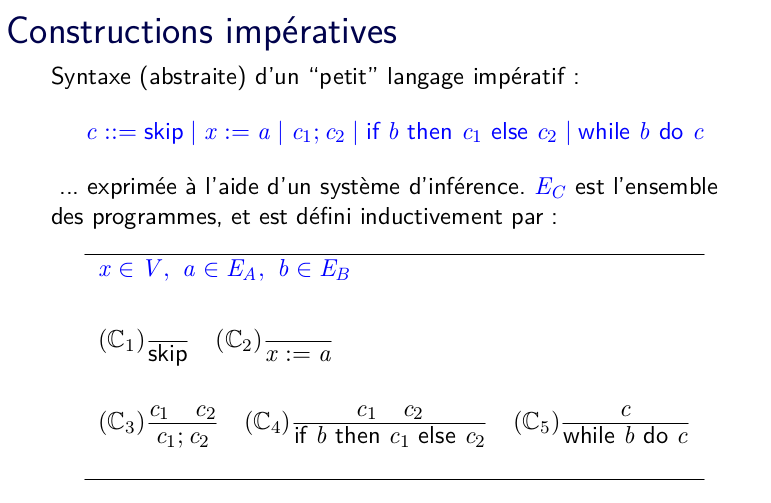
\includegraphics[height=4cm]{\IMProot/definition_inductive.png} \\
A présent, nous allons pouvoir écrire des programmes impératifs !

	\subsection{Traduction en OCaml}
	\lstinputlisting[language=OCaml, linerange={454-456, 463-463, 502-508}]{\OCamlroot/OCaml_exemple.ml}

	\subsection{Traduction en K}
	\lstinputlisting[language=K, linerange={86-97}]{K_SemantiK/K_exemple.k}




\section{Sémantique opérationnelle d’évaluation à grands pas}

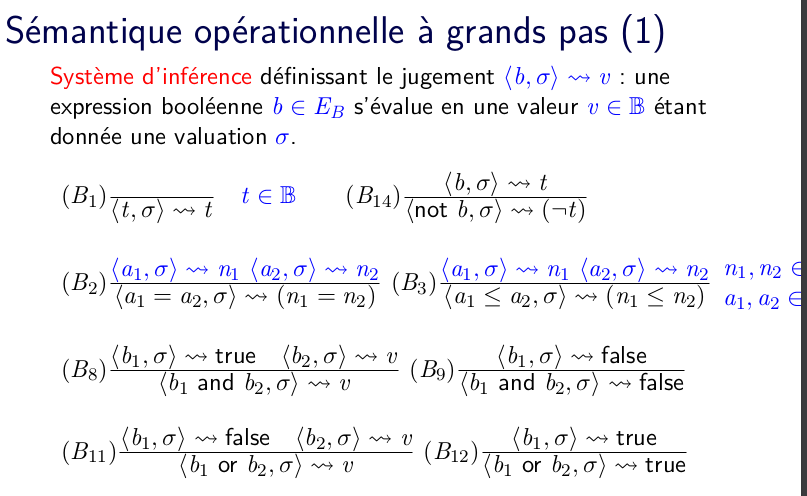
\includegraphics[height=4cm]{\IMProot/eval_grands_pas.png}


\section{Sémantique opérationnelle d’évaluation à petits pas}

	\subsection{Traduction en OCaml}

\lstinputlisting[language=OCaml, linerange={510-514}]{\OCamlroot/OCaml_exemple.ml}


\lstinputlisting[language=OCaml, linerange={526-537}]{\OCamlroot/OCaml_exemple.ml}

\lstinputlisting[language=OCaml, linerange={565-570}]{\OCamlroot/OCaml_exemple.ml}


\subsection{Traduction en K}
\lstinputlisting[language=K, linerange={99-124}]{K_SemantiK/K_exemple.k}